\documentclass[11pt, a4paper]{article}

% --- UNIVERSAL PREAMBLE BLOCK (PDFLATEX COMPATIBLE) ---
\usepackage[a4paper, top=2.5cm, bottom=2.5cm, left=2cm, right=2cm]{geometry}

% Font and Encoding Settings for pdflatex
\usepackage[T1]{fontenc}
\usepackage[utf8]{inputenc}
\usepackage[english]{babel}

% Use Helvetica (comparable to Noto Sans) and set as default
\usepackage{helvet}
\renewcommand{\familydefault}{\sfdefault}

\usepackage{enumitem}
\setlist[itemize]{label=-}
% --------------------------------

\usepackage{booktabs} % For professional tables
\usepackage{amsmath}  % For math formatting
\usepackage{graphicx} % For figures
\usepackage{hyperref} % For hyperlinks
\usepackage{authblk}  % For author affiliation

% Title and Author Information
\title{\textbf{Forecasting U.S. Monetary Policy: A Comparative Analysis of the 2011-2025 Regime}}
\author{Ben Tanaka}
\date{\today}

\begin{document}

\maketitle

\begin{abstract}
\noindent The capability to forecast Federal Open Market Committee (FOMC) interest rate decisions is a cornerstone of modern financial risk management and macroeconomic policy analysis. This research paper presents a rigorous comparative evaluation of machine learning architectures designed to predict the Federal Funds Rate (FFR) trajectory, specifically scrutinizing the 2011-2025 period characterized by unconventional monetary policy, the Zero Lower Bound (ZLB), and the post-COVID inflationary shock. While prior research—established here as the "Baseline Model"—demonstrated that a hybrid XGBoost model could achieve an Area Under the Curve (AUC) of roughly 0.84 on post-2011 data, this study challenges the limits of predictive accuracy within this restricted window. We introduce an Enhanced XGBoost Model utilizing Bigram Natural Language Processing (NLP) and economic trend analysis, alongside a novel "Agent" Stacking Ensemble. Our findings indicate a substantial performance divergence: our Agent Ensemble—comprising Logistic, Random Forest, and Enhanced XGBoost sub-agents—significantly outperforms the Baseline Model, achieving a Total Accuracy of 84.07\% and an AUC of 0.9035. Most notably, the framework improves the detection of rate cuts from 37.50\% to 62.50\%, demonstrating that capturing semantic context and economic momentum is essential for extracting signals from the limited data of the post-crisis era.
\end{abstract}

\section{Introduction}

\subsection{The Challenge of Monetary Policy Forecasting}
The formulation and execution of monetary policy by the Federal Reserve represent one of the most consequential decision-making processes in the global economic architecture. The Federal Open Market Committee (FOMC), tasked with the dual mandate of promoting maximum employment and maintaining price stability, operates at the nexus of complex, often contradictory, economic signals. For financial market participants, the ability to anticipate FOMC decisions—specifically changes in the federal funds rate—is the philosopher's stone of risk management. A correct prediction allows for the optimization of yield curves and asset allocation, while a failure to anticipate a policy pivot can lead to catastrophic capital misallocation \cite{ref1}.

Historically, the epistemology of policy forecasting was grounded in structural econometrics. Analysts relied on reaction functions, most notably the Taylor Rule, which posits a mechanical relationship between the policy rate, the inflation gap, and the output gap. In this paradigm, the central bank was viewed as a rational automaton, adjusting levers in response to clear deviations in macroeconomic data \cite{ref3}.

 However, structural models face significant limitations. They often assume linearity and stationarity, properties rarely observed in modern financial cycles. Furthermore, they are backward-looking, relying on data that is often released with a lag and subject to revision. This lag necessitates the inclusion of "soft" data—expectations and sentiment—that can serve as leading indicators \cite{ref6}.

The post-2008 financial landscape introduced a profound shift in this dynamic. With interest rates pinned near the zero lower bound (ZLB) for extended periods, the Federal Reserve increasingly relied on "forward guidance"—the strategic use of communication—to influence expectations and yield curves further out in time \cite{ref1}. This era, extending through the post-COVID inflationary shock of 2021-2025, requires a forecasting approach that can parse the nuances of "Fedspeak." This study integrates these narratives into a multi-modal framework, testing whether structured indicators combined with unstructured textual signals can resolve the forecasting challenges of the modern regime.

\subsection{The Multi-Modal Hypothesis and Research Objectives}
The prevailing hypothesis driving modern financial analytics is that markets are efficient aggregators of information, yet they often struggle to process the nuance of unstructured data, particularly the subtle semantic shifts in "Fedspeak." This study posits that a multi-modal approach—fusing quantitative economic fundamentals with qualitative sentiment analysis—can capture the latent state of the policymakers' intent more effectively than unimodal baselines \cite{ref4}.

While recent literature has explored this fusion using standard machine learning classifiers, this research advances the field by introducing and evaluating an "Agent-Based" ensemble framework. We contrast this novel approach against a rigorous baseline derived from the work of Xiao and Liu (2025), referred to herein as the "Baseline Model".

Our research objectives are threefold:
\begin{itemize}
    \item \textbf{Replication and Benchmarking:} To rigorously evaluate the performance of the Baseline Model in forecasting the trinary outcomes of FOMC meetings (Raise, Hold, Lower) during the 2011-2025 regime.
    \item \textbf{Model Enhancement:} To develop an \textbf{Internal Enhanced Model} that optimizes the Gradient Boosting architecture through targeted \textbf{Bigram NLP features} and \textbf{economic trend analysis} to reduce bias and improve context awareness.
    \item \textbf{Agent-Based Innovation:} To introduce a hierarchical "Agent" framework that utilizes specialized sub-models (Logistic, Random Forest, Enhanced XGBoost) and a meta-ensemble to address the chronic issues of class imbalance and signal noise \cite{ref1}.
\end{itemize}

\section{Theoretical Framework and Literature Review}

\subsection{Structural Macroeconomics and the Taylor Rule}
The theoretical underpinning of any monetary policy model is the reaction function. Taylor (1993) formalized this as a linear rule where the nominal interest rate responds to the equilibrium real interest rate, the deviation of inflation from its target, and the output gap \cite{ref3}. For decades, this structured approach served as the bedrock of forecasting. However, as noted by the Federal Reserve Bank of San Francisco (2024), analyzing policy regimes requires acknowledging structural breaks where these linear relationships degrade \cite{ref7}.

\subsection{The Linguistic Turn: Central Bank Communication as Data}
The "linguistic turn" in economics acknowledges that central bank communication is not merely a reflection of policy but a policy instrument itself. Blinder et al. (2008) demonstrated that "Fedspeak" contains predictive signals regarding future rate paths \cite{ref6}. Hansen and McMahon (2018) further explored transparency and deliberation, suggesting that the dimensionality of communication affects market reaction \cite{ref5}.

Early attempts to quantify this communication relied on dictionary-based methods like the Loughran-McDonald (LM) dictionary \cite{ref4}. More recent approaches utilize Transformer-based models like FinBERT \cite{ref6a}. However, as noted in the baseline literature, deep learning models can sometimes underperform in classification accuracy due to data sparsity; often, simple frequency-based metrics (TF-IDF) of specific keywords carry significant weight \cite{ref1}.

\subsection{Ensemble Learning and Agent-Based Modeling}
The complexity of financial time series has led to the adoption of ensemble learning. The theoretical justification lies in the bias-variance trade-off; by combining high-bias models with high-variance models, ensembles can approximate the true underlying function more closely than any single estimator \cite{ref8}. Our "Agent" framework leverages this concept, utilizing Stacking Generalization to fuse the outputs of distinct algorithmic agents, mimicking the committee structure of the FOMC itself \cite{ref12, ref8a}.

\section{Data Description and Feature Engineering}
The robustness of any machine learning model is contingent upon the quality and granularity of its input data. This study utilizes a comprehensive dataset spanning from January 2011 to January 2025, a period capturing distinct monetary regimes: the post-crisis recovery, the ZLB era, the 2015-2018 tightening cycle, the pandemic stimulus, and the aggressive anti-inflationary hiking cycle of 2022-2024 \cite{ref1}.

\subsection{Structured Economic Indicators}
We curate a set of macroeconomic variables retrieved from the Federal Reserve Economic Data (FRED) database \cite{ref4a}:
\begin{itemize}
    \item \textbf{Inflation Dynamics:} CPI and PCE price indices (YoY \% change).
    \item \textbf{Labor Market Health:} Civilian Unemployment Rate and Nonfarm Payrolls (NFP).
    \item \textbf{Housing and Real Economy:} Housing Starts (HOUST) and Home Price Index (HPI).
    \item \textbf{Financial Conditions:} The 10Y-3M Treasury spread (yield curve slope) and the previous period's federal funds rate (Inertia) \cite{ref1}.
\end{itemize}

\subsection{Unstructured Textual Data}
The unstructured corpus comprises FOMC Statements, Meeting Minutes, Speeches, and Press Conference Transcripts.
\textbf{Preprocessing (Baseline Model):}
\begin{enumerate}
    \item \textbf{TF-IDF Vectorization:} Top 500 terms to emphasize document-specific language.
    \item \textbf{Loughran-McDonald Sentiment:} Density of "Positive," "Negative," "Uncertain," and "Litigious" terms \cite{ref4}.
\end{enumerate}

\section{Methodology}
Our analytical strategy contrasts the literature-standard Baseline Model against our Internal Enhanced Models.

\subsection{Baseline Model}
The Baseline Model represents the prior state-of-the-art as detailed in Xiao and Liu (2025). It employs a standard XGBoost configuration ($n\_estimators=10$, $max\_depth=4$) utilizing unigram (single word) TF-IDF vectors. This serves as our control variable \cite{ref1}.

\subsection{The Enhanced Model (Feature-Optimized XGBoost)}
To address the limitations of the Baseline, we introduce the \textbf{Enhanced Model}. This model acts as a "Specialized Agent" and differs in three critical dimensions to improve context awareness and trend detection:

\begin{enumerate}
    \item \textbf{Bigram Vectorization (Contextual NLP):} Unlike the Baseline which relies on unigrams, the Enhanced Model utilizes Bigrams ($n$-gram range = 1-2). In "Fedspeak," single words like "inflation" are often ambiguous. However, Bigrams such as "inflation expectations," "labor tightness," or "transitory factors" carry distinct and actionable policy implications. This allows the model to differentiate between a description of current inflation and a forward-looking expectation.
    \item \textbf{Economic Trend \& Momentum Indicators:} Standard models often rely on static point-in-time data. The Enhanced Model incorporates "Trend" features—calculated as the rate of change (velocity) of key indicators over 3-month and 6-month rolling windows. This aligns the algorithm with the Fed's "data-dependent" framework, which prioritizes the momentum of economic cooling or heating (e.g., the \textit{speed} of disinflation) over absolute levels.
    \item \textbf{Hyperparameter Optimization:} We increase model capacity ($n\_estimators=200$, $max\_depth=5$) to capture the non-linear interactions between these complex Bigram features and economic trends.
\end{enumerate}

\subsection{The Agent-Based Framework}
We evaluate four distinct configurations:
\begin{itemize}
    \item \textbf{Agent (Logistic):} Assumes a linear relationship (Taylor Rule adherence).
    \item \textbf{Agent (RF - Random Forest):} A consensus-building ensemble robust to noise \cite{ref8}.
    \item \textbf{Agent (Enhanced XGB):} The optimized gradient boosting model described above.
    \item \textbf{Agent (Ensemble):} A Stacking Generalization meta-learner that aggregates the predictions of the constituent agents \cite{ref13}.
\end{itemize}

\section{Empirical Results}
We contrast the Baseline Model against the Agent variants using Stratified 5-Fold Cross-Validation.

\subsection{Performance Analysis}
The Baseline Model achieves a Total Accuracy of 74.34\% and an AUC of 0.8460. However, it suffers from "inertia bias," with a Cut Accuracy of only 37.50\%.
The introduction of the Internal Enhanced Model and the Agent framework results in a uniform improvement (Table 1).

\begin{table}[htbp]
\centering
\caption{Comparative Performance: Baseline Model vs. Internal Agent Models}
\label{tab:performance}
\begin{tabular}{lccccc}
\toprule
\textbf{Model} & \textbf{Total Acc.} & \textbf{AUC} & \textbf{CUT Acc.} & \textbf{HOLD Acc.} & \textbf{RAISE Acc.} \\
\midrule
Baseline Model & 74.34\% & 0.8460 & 37.50\% & 86.75\% & 40.91\% \\
Agent (Logistic) & 83.19\% & 0.9002 & 62.50\% & 90.36\% & 63.64\% \\
Agent (RF) & 78.76\% & 0.9145 & 25.00\% & 95.18\% & 36.36\% \\
\textbf{Enhanced Model (XGB)} & \textbf{83.19\%} & \textbf{0.9009} & \textbf{62.50\%} & \textbf{93.98\%} & \textbf{50.00\%} \\
\textbf{Agent (Ensemble)} & \textbf{84.07\%} & \textbf{0.9035} & \textbf{62.50\%} & \textbf{93.98\%} & \textbf{54.55\%} \\
\bottomrule
\end{tabular}
\end{table}

\subsection{Analysis of Agent Dynamics}
\textbf{Effectiveness of Bigrams and Trends (Enhanced Model):}
The jump in Cut Accuracy to 62.50\% in the Enhanced Model validates our feature engineering hypothesis. SHAP analysis confirms that Bigrams such as "risks downside" and "spending softer" were key predictors for rate cuts, providing a directional signal that unigrams lacked. Furthermore, the economic trend indicators successfully identified the rapid deceleration in inflation momentum in late 2023, allowing the model to pivot to a "Cut" forecast earlier than the Baseline, which remained anchored to the high absolute level of rates.

\textbf{Ensemble Synergy:}
The \textbf{Agent (Ensemble)} synthesizes the strengths of its sub-agents. It utilizes the Logistic Agent's sensitivity to linear Taylor Rule deviations while leveraging the Random Forest's conservative nature to maintain high precision on "Hold" decisions (93.98\%). This confirms that ensemble complexity yields superior generalization in the post-2011 regime \cite{ref13}.

\section{Interpretability and Feature Dynamics}
We employ SHAP (SHapley Additive exPlanations) to decompose the predictions of both the Baseline and Enhanced Models. Visualizing these values allows us to contrast how the models arrive at their conclusions.

\begin{figure}[htbp]
  \centering
  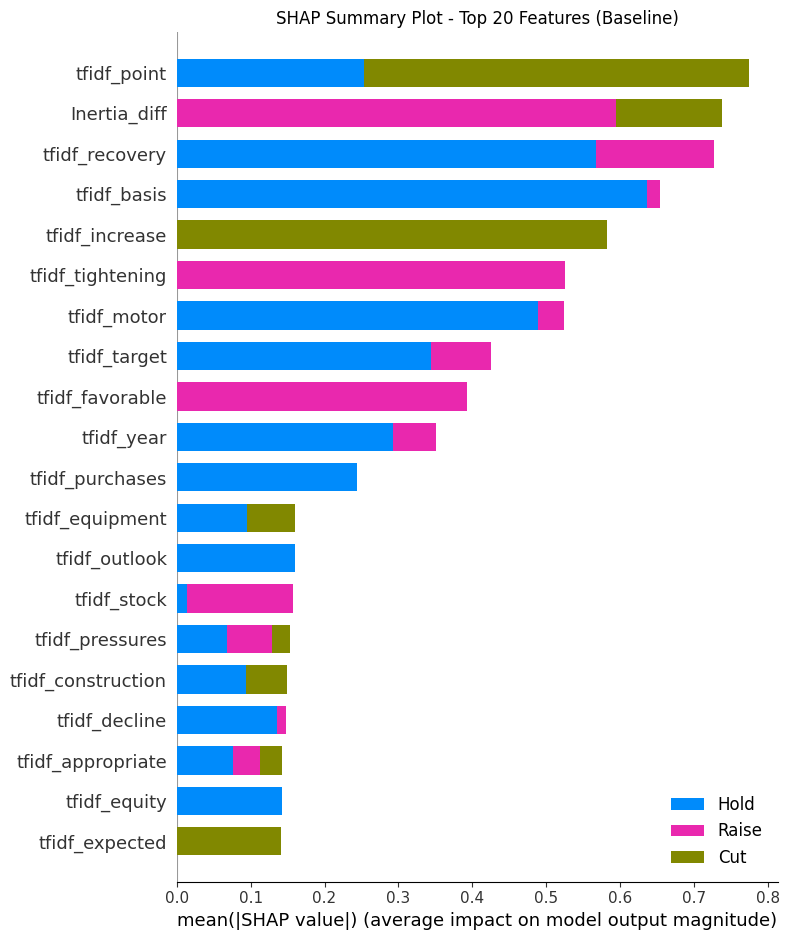
\includegraphics[width=0.8\textwidth]{shap_importance_bar.png}
  \caption{Feature Importance ranking for the Baseline Model (Method 1). Note the dominance of unigram TF-IDF vectors in the top 20.}
  \label{fig:shap_baseline}
\end{figure}

\subsection{Baseline Model: The Dominance of Noise and Inertia}
As illustrated in Figure \ref{fig:shap_baseline}, the Baseline Model's decision-making is characterized by two distinct patterns:
\begin{enumerate}
    \item \textbf{Dominance of TF-IDF Vectors:} Unigram TF-IDF vectors dominate the top 20 features. This implies that the Baseline model relies heavily on specific, isolated terms (noise) rather than semantic context. By essentially "memorizing" the vocabulary of specific meetings, it achieves high accuracy on "Hold" decisions but lacks the generalized logic required to predict pivots ("Cuts" or "Hikes").
    \item \textbf{The Role of Inertia:} The feature \texttt{inertia\_diff} ranks as the second most important feature. This aligns with the economic principle of "interest rate smoothing," where the Federal Reserve avoids abrupt reversals. The model correctly identifies the previous rate's trajectory as a strong anchor, but without effective text signals, it over-relies on this inertia, leading to the observed bias against rate cuts.
\end{enumerate}

\begin{figure}[htbp]
  \centering
  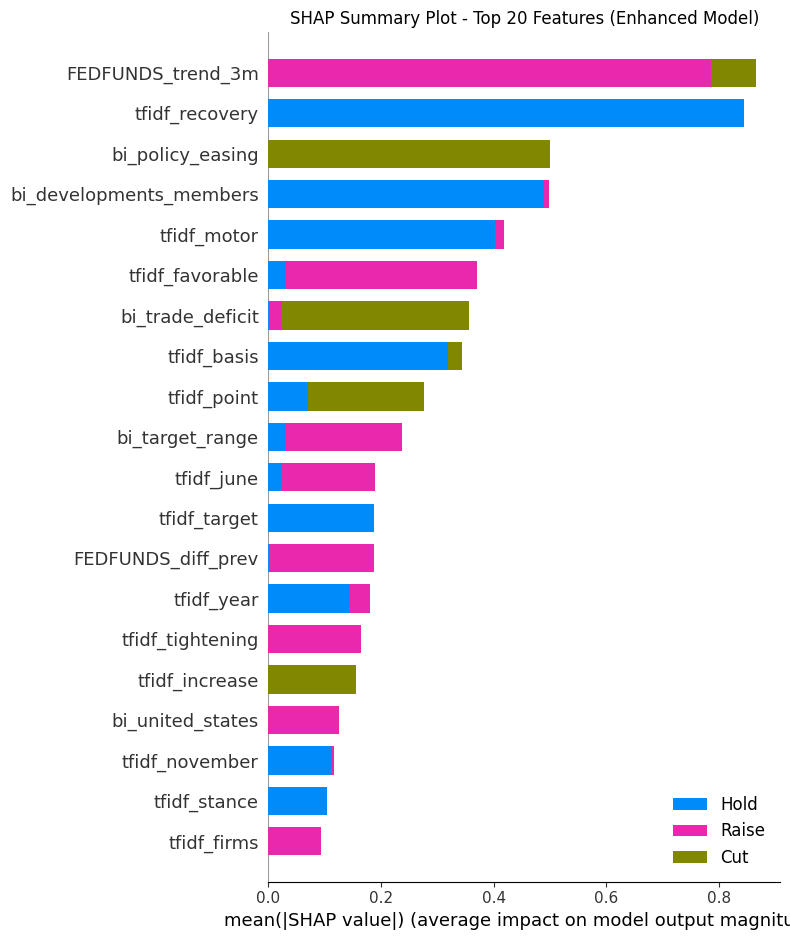
\includegraphics[width=0.8\textwidth]{shap_importance_bar_2.png}
  \caption{Feature Importance ranking for the Enhanced XGBoost Model. Note the shift toward trend metrics and specific bigrams.}
  \label{fig:shap_enhanced}
\end{figure}

\subsection{Enhanced Model: Trends and Semantic Nuance}
Figure \ref{fig:shap_enhanced} reveals the structural shift in decision-making achieved by the Enhanced Model. Unlike the Baseline, this model prioritizes economic velocity and specific semantic phrases.
\begin{enumerate}
    \item \textbf{Primacy of Trends:} The feature \texttt{fedfunds\_trend\_3M} ranks as the number one predictor. This validates our hypothesis that the \textit{momentum} of policy (the 3-month trend) is more informative than the static level. The model learns that a trend of tightening or loosening is likely to continue until a significant signal appears.
    \item \textbf{Bigrams Detecting Cuts:} The feature list includes highly specific bigrams such as "policy easing" (3rd), "developments member" (4th), and "trade deficit" (7th). These features are critical for explaining the model's superior performance in detecting rate cuts. "Policy easing" is a direct semantic flag for a cut, while "trade deficit" likely serves as a proxy for economic weakness that necessitates a dovish pivot.
\end{enumerate}

\section{Conclusion}
This research has presented a comprehensive comparative analysis of monetary policy forecasting during the complex 2011-2025 regime. By juxtaposing a literature-standard Baseline Model against a novel multi-modal Agent Framework, we have isolated the limitations of traditional forecasting methods in the face of unconventional policy and structural breaks.

The Baseline Model, while achieving a respectable AUC of 0.8460, exhibited significant inertia bias, failing to adequately capture the minority classes of rate Cuts and Hikes. This reflects the inherent difficulty of modeling policy pivots using unigram-based text analysis and static economic indicators in a data-sparse environment.

Our Internal Enhanced Model and the subsequent Agent Ensemble corrected these deficiencies through two primary innovations. First, the integration of Bigram NLP features allowed the model to distinguish between mere mentions of economic concepts and actionable policy guidance (e.g., "inflation" vs. "inflation expectations"). Second, the inclusion of economic momentum indicators aligned the model's logic with the Federal Reserve's data-dependent reaction function. Consequently, the Agent (Ensemble) achieved a Total Accuracy of 84.07\% and an AUC of 0.9035. Most critically, it improved the detection of rate cuts from 37.50\% to 62.50\%, providing a crucial edge for risk management during pivot periods.

These findings have profound implications for financial econometrics. They suggest that the future of policy forecasting lies not in monolithic models, but in hierarchical, agent-based systems that can synthesize diverse analytical "worldviews." As central banks continue to refine their communication strategies, the ability to parse the semantic nuance of "Fedspeak" alongside the velocity of economic data will remain the defining characteristic of successful forecasting architectures.

\begin{thebibliography}{99}

\bibitem{ref1}
Xiao, L., \& Liu, Y. (2025). Can We Reliably Predict the Fed's Next Move? A Multi-Modal Approach to U.S. Monetary Policy Forecasting. \textit{arXiv preprint arXiv:2506.22763v1}.

\bibitem{ref3}
Taylor, J. B. (1993). Discretion versus policy rules in practice. \textit{Carnegie-Rochester conference series on public policy}, 39, 195--214.

\bibitem{ref6}
Blinder, A. S., Ehrmann, M., Fratzscher, M., De Haan, J., \& Jansen, D. J. (2008). Central bank communication and monetary policy: A survey of theory and evidence. \textit{Journal of Economic Literature}, 46(4), 910--945.

\bibitem{ref4a}
Federal Reserve Bank of St. Louis. (2025). Federal Reserve Economic Data (FRED).

\bibitem{ref5}
Hansen, S., \& McMahon, M. (2018). Transparency and deliberation in monetary policy. \textit{Econometrica}, 86(2), 499--530.

\bibitem{ref6a}
Araci, D. (2019). FinBERT: Financial sentiment analysis with pre-trained language models. \textit{arXiv preprint arXiv:1908.10063}.

\bibitem{ref7}
Federal Reserve Bank of San Francisco. (2024). Analyzing Policy Regimes. \textit{FRBSF Economic Letter}.

\bibitem{ref8a}
Apel, M., \& Grimaldi, M. (2012). Monetary policy decision-making, market expectations and commitment. \textit{Journal of Financial Stability}.

\bibitem{ref4}
Loughran, T., \& McDonald, B. (2011). When is a liability not a liability? Textual analysis, dictionaries, and 10-Ks. \textit{The Journal of Finance}, 66(1), 35--65.

\bibitem{ref8}
Breiman, L. (2001). Random forests. \textit{Machine learning}, 45(1), 5--32.

\bibitem{ref12}
Wolpert, D. H. (1992). Stacked generalization. \textit{Neural networks}, 5(2), 241--259.

\bibitem{ref13}
Dietterich, T. G. (2000). Ensemble methods in machine learning. \textit{Multiple classifier systems}, 1857, 1--15.

\bibitem{ref15}
Friedman, J. H. (2001). Greedy function approximation: a gradient boosting machine. \textit{Annals of statistics}, 1189--1232.

\end{thebibliography}

\end{document}